\section{Практычны занятак №4}

\subsection{Структура праекта}

На малюнку \ref{img: pz4} прадстаўлена файлавая структура праекта.

\begin{figure}[h!]
\centering
\begin{subfigure}{0.5\textwidth}
    \centering
   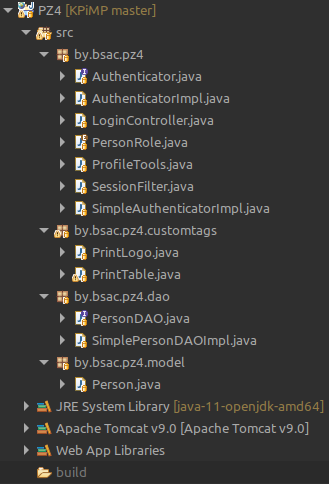
\includegraphics[width=\textwidth]{pz4_structure_1}
\end{subfigure}%
\begin{subfigure}{0.5\textwidth}
    \centering
    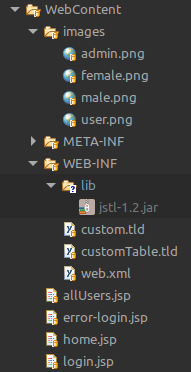
\includegraphics[width=0.7\textwidth]{pz4_structure_2}
\end{subfigure}
\caption{Файлавая структура практычнага занятку}
\label{img: pz4} 
\end{figure}

\subsection{Заданне з тэорыі}

Дадзенае заданне выконваецца на базе прыктачнага занятка №3
(заданне з тэорыі).

\subsubsection{Апісанне задання.}

Арганізаваць вывад лагатыпа карыстальніка пры дапамозе карыстальніцкіх
тэгаў.

Для гэтага перад тым, як пачаць выконваць задання, неабходна
пакласці карцінкі лагатыпаў у \textit{WebContent/images}.

\subsection{Зыходны код. Java}

\subsubsection{Клас PrintLogo.}

Дадзены клас адказвае за выкананне дзеянняў (пабудова поўнага шляху
да карцінкі лагатыпа) пры выкліку тэга ў JSP старонцы.

У лістынгу \ref{lst: pz4_printLogo} прадстаўлены зыходны код класа \textit{PrintLogo}.

\lstinputlisting[caption={Зыходны код класа PrintLogo},%
                 label={lst: pz4_printLogo},%
                 language=java]{PZ4/Java/PrintLogo.java}

\vspace{-\baselineskip}
\subsubsection{Канфігурацыя тэга custom.tld.}

Для таго, каб вэб-праграма ведала пра створаны тэг, неабходна
апісаць яго. Для гэтага апішам тэг у файле \textit{custom.tld} і
пакладзем яго ў \textit{WEB-INF}.

У лістынгу \ref{lst: pz4_custom} прадстаўлена апісанне \textit{custom.tld}.

\lstinputlisting[caption={Апісанне custom.tld},%
                 label={lst: pz4_custom},%
                 language=java]{PZ4/custom.tld}

\vspace{-\baselineskip}
\subsubsection{Абноўленая старонка home.jsp}

Абнавім старонку \textit{home.jsp}, каб на ёй выводзіўся лагатып
карыстальніка; шлях лагатыпа ствараўся пры дапамозе карыстальніцкага
тэга.

У лістынгу \ref{lst: pz4_home} прадстаўлена абноўленая старонка \textit{home.jsp}.

\lstinputlisting[caption={Старонка home.jsp},%
                 label={lst: pz4_home},%
                 language=HTML5,%
                 style=htmlcssjs]{PZ4/JSP/home.jsp}

\subsection{Індывідуальнае заданне}

\subsubsection{Апісанне задання.}

На старонцы \textit{allUsers.jsp} табліцу \textit{users} вывесці
пры дапамозе карыстальніцкага тэга.

\subsubsection{Клас PrintTable}

Як было апісана вышэй, для рэалізацыі карыстальніцкага тэга неабходна
стварыць клас, які будзе вызначаць логіку тэга.

У лістынгу \ref{lst: pz4_printTable} прадстаўлены зыходны код абноўленага класа \textit{PrintTable}.

\lstinputlisting[caption={Зыходны код класа PrintTable},%
                 label={lst: pz4_printTable},%
                 language=java]{PZ4/Java/PrintTable.java}

\subsubsection{Апісанне тэга customTable.tld.}

У лістынгу \ref{lst: pz4_customTable} прадстаўлена апісанне тэга \textit{customTable.tld}.

\lstinputlisting[caption={Апісанне тэга customTable.tld},%
                 label={lst: pz4_customTable},%
                 language=HTML5,%
                 style=htmlcssjs]{PZ4/customTable.tld}

\subsubsection{Абноўленая старонка allUsers.jsp}

Заменім стварэнне табліцы карыстальнікаў у самой старонцы
на выклік уласнага тэга.


У лістынгу \ref{lst: pz4_allUsers} прадстаўлена абноўленая старонка \textit{allUsers.jsp}.

\lstinputlisting[caption={Старонка allUsers.jsp},%
                 label={lst: pz4_allUsers},%
                 language=HTML5,%
                 style=htmlcssjs]{PZ4/JSP/allUsers.jsp}
